\documentclass[english]{article}

\usepackage{graphicx}
\usepackage{grffile}
\usepackage[T1]{fontenc}
\usepackage{babel}
\usepackage{wrapfig}
\usepackage{hyperref}

\date{\today}

\graphicspath{{Pictures/}}
\begin{document}	
	\begin{titlepage}
		\pagenumbering{gobble}
		\begin{figure}[!t]
			
\includegraphics[width=\linewidth]{up_logo.png}
		\end{figure}
		\vspace*{\stretch{1.0}}
		\begin{center}
			\huge{Project: Harvest}\\
			\large{Client: Subtrop}\\
			\vspace{10mm}
			\huge{Team: A-Cube-N}\\
		\end{center}
		\begin{center}
			\begin{tabular}{ c c c }
				Dunkley, Nathan & Grobler, Arno & Lochner, Amy \\
				\texttt{14145759} & \texttt{14011396} & \texttt{14038600}\\
				& Maree, Armand &\\
				& \texttt{12017800} &
			\end{tabular}
		\end{center}
		\begin{center}
			Department of Computer Science, University of Pretoria
		\end{center}
		\begin{center}
			\today
			\begin{figure}[!h]
				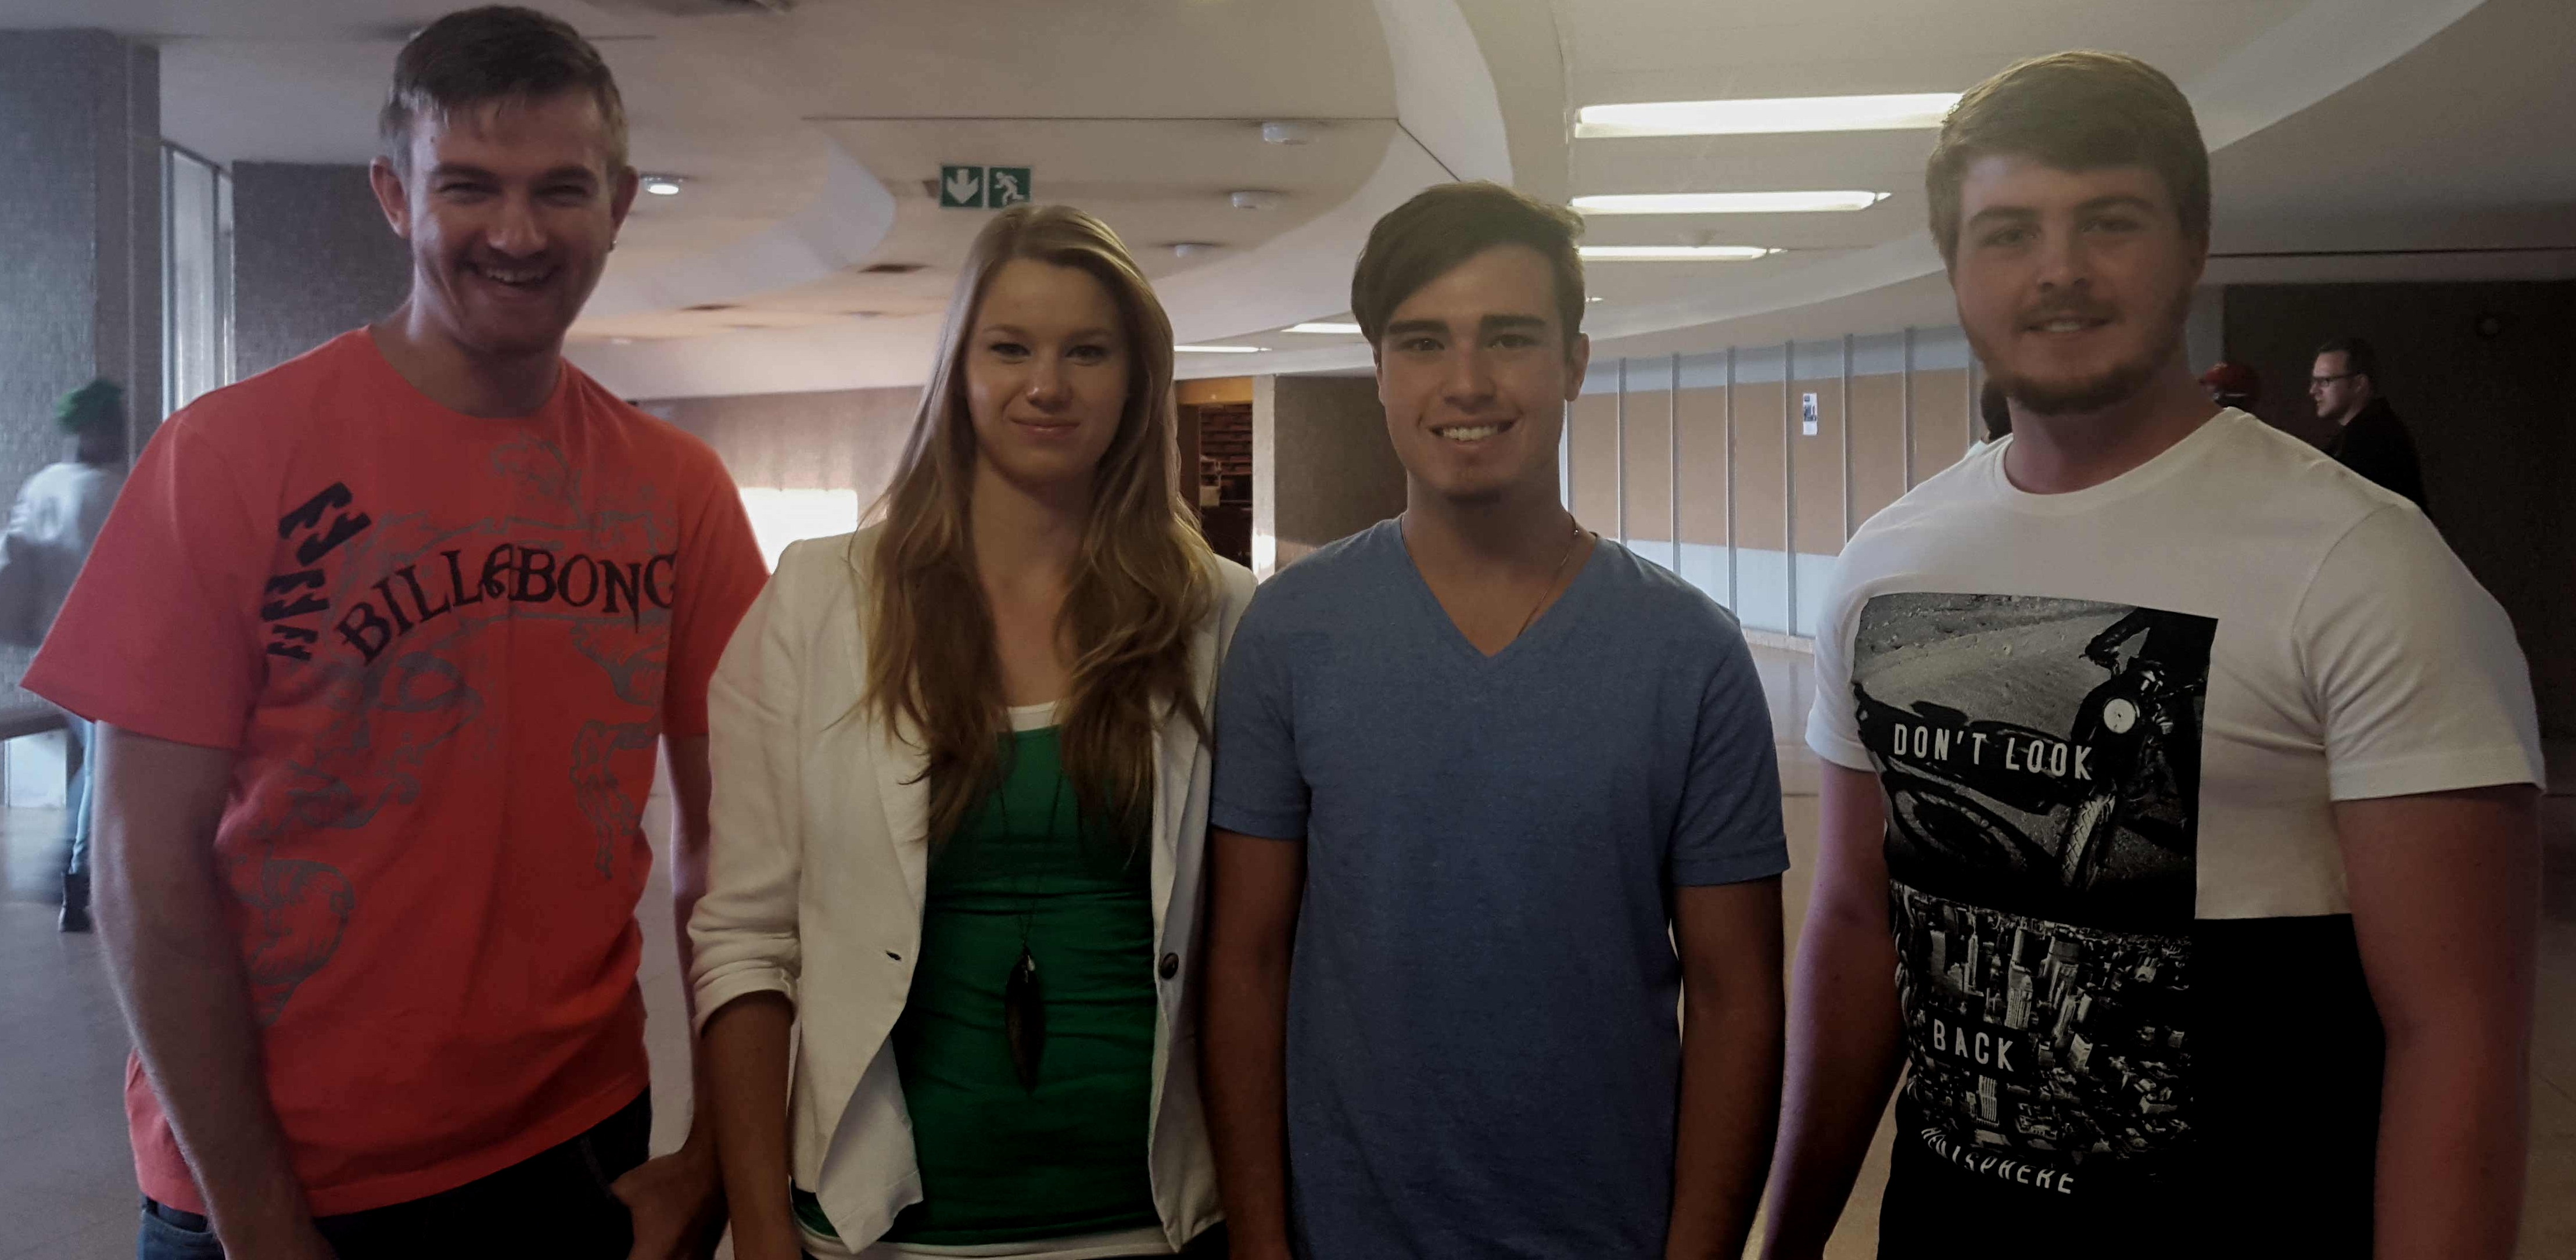
\includegraphics[width=\linewidth]{team.jpg}
			\end{figure}
		\end{center}
		\vspace*{\stretch{2.0}}
	\end{titlepage}
	\newpage
	\tableofcontents
	\newpage
	\pagenumbering{arabic}
	\section{The Team}
		\subsection{Nathan Dunkley}
		
		\subsection{Arno Gerber}
		\begin{wrapfigure}{l}{5.1cm}
			\begin{center}
				
\includegraphics[width=5cm]{arno.jpg}
			\end{center}
		\end{wrapfigure}
		\paragraph{Interests and Hobbies}
		My interests include collecting music, long distance running, painting and drawing, reading, computer games and obviously spending most of my days programming. Not only do I want to program as a profession, it is also a hobby for me. Integrating my other hobbies into my programming is my passion.
		
		\paragraph{Technical Skills}
		I pride myself in always looking for new skills and for me, learning a new technical skill is the best part of the experience. I enjoy making my projects look visually pleasing and spend as much time making a working, functional program as I do making it look good. I have good logical and problem solving skills and enjoy problems presented to me in computer science. My technical skills stem from Mathematics and computer science, especially those skills from data structures and algorithms and programming logic.
		
		\paragraph{Past Experience}
		I have created static websites for companies before, my most recent one is (\href{http://bodytalkbethlehem.com/}{http://bodytalkbethlehem.com/}) and (\href{http://honeydewpools.co.nf/}{http://honeydewpools.co.nf/}).
		
		\paragraph{Non-Technical Strengths}
		\begin{itemize}
			\setlength\itemsep{0.2em}
			\item Eager learner
			\item Organised 
			\item Good time management
			\item Good communication skills
			\item Creative
		\end{itemize}
		
		\paragraph{Motivation}
		The most appealing part of this project was the huge practical implications of having this system developed for the agricultural industry. Developing a project that a person knows is going to be used and has a use in today’s world increases the motivation of the person developing the software. The technologies that were requested is also appealing as I have always wanted to make a cross platform application.
		
		\subsection{Amy Lochner}
		\begin{wrapfigure}{l}{5cm}
			\begin{center}
				
\includegraphics[width=8cm, height=4.5cm, angle=90]{amy.jpg}
			\end{center}
		\end{wrapfigure}
		\paragraph{Interests and Hobbies}
		My interests include music, classic cars, cooking, traveling, breeding Shetland sheepdogs. My hobbies include reading, playing piano, camping, 4x4ing, tennis, training my dog, mountain biking and horse riding.
		
		\paragraph{Technical Skills}
		I am good at determining functional requirements of a system. I can place myself in the users shoes, this is valuable when determining how the user will intend to use a system. I can follow business logic easily and I have experience in databasing, Informatics, Statistics, Mathematics, multiple programming languages and Human Computer Interaction.
		
		\paragraph{Past Experience}
		I have built a fully functional, responsive website. I have helped a company modify their website. I have also observed (by job shadowing) the process of creating a system for a business and have noticed which qualities have caused them to excel and which have caused them to fail. I intend to use that knowledge to keep our team constantly progressing forward.
		
		\paragraph{Non-Technical Strengths}
		\begin{itemize}
			\setlength\itemsep{0.2em}
			\item Organized
			\item Good at prioritising 
			\item Team player
			\item Good leader
			\item Optimistic
			\item Quick learner
			\item Determined
		\end{itemize}
		
		\paragraph{Motivation}
		When I first read this project proposal I took an instant liking to the project. The whole idea of modernising a management system for subtropical farmers sounded like an amazing opportunity. I especially liked the fact that no explicit technological requirements were stated; I feel that this will allow us to be very creative and provide a system best suited to the needs of the farmers. I was ecstatic to here Subtrop wished for the project to be open source; thus allowing anyone to benefit from it. I felt that showed great generosity and kindness. I know that the farming industry is possibly one of the most important industries that contribute to the economy but also contribute to society by providing natural produce. I feel many people overlook the importance of farmers, and I have had a lot of experience in Non-profit organisations -as I went to an NPO school- and I know some of the hardships and struggles that are often presented to NPOs and therefore I would feel honored to be part of the team selected to help the farmers in Subtrop join the mobile community.
		
		\subsection{Armand Maree}
			\begin{wrapfigure}{l}{5.1cm}
				\begin{center}
					
\includegraphics[width=5cm]{armand.jpg}
				\end{center}
			\end{wrapfigure}
			\paragraph{Interests and Hobbies}
			During my off time I like to socialize with friends and enjoy watching sports. I also like solving puzzles to keep my brain active during holidays.\\
			Tutoring scholars and university students has become a passion for me. I always look forward to these sessions.
			
			\paragraph{Technical Skills}
			I am good at solving complex problems and building data structures. I believe this is a valuable skill to complete any project, especially in the field of computer science.
			
			\paragraph{Past Experience}
			I have developed websites for other start up companies and I also have a website of my own (\href{http://www.codehaven.co.za}{www.codehaven.co.za}). I also have some Android developing experience I gained from side projects.
			
			\paragraph{Non-Technical Strengths}
			\begin{itemize}
				\setlength\itemsep{0.2em}
				\item Good leader
				\item Fast learner
				\item Team player
				\item Good communicator
				\item Passionate
				\item Problem solver
			\end{itemize}
			
			\paragraph{Motivation}
			As soon as I read the project specifictions I was very eager to apply for it. The most attractive part of the project was the fact that is so applicable to the industry. Developing a system that would directly help the country, and more specifically farmers, sounded like a great idea. Since I am also a huge advocate of open source software, the proposal by Subtrop to make this software available for other farmers was a big attraction.
			
	\newpage
	\section{Project Execution}
		\subsection{Development Methodology}
			\paragraph\indent
			We are planning on using the Agile iterative software development methodology. The reason we have chosen this methodology can be described through the benefits of this methodology:
			\begin{itemize}
				\setlength\itemsep{0.2em}
				\item High degree of collaboration between the client and project team
				\item Allows clients to be involved throughout the project - this requires clients to understand that the work they will see is a 'work in progress'
				\item By using the idea of Sprints new features are delivered quickly and frequently
				\item Focusing on users needs results in each feature incrementally delivering value not only an IT component
				\item The breaking down of the projects into units allows the team to focus of high-quality development, testing and collaboration. Quality is improved by finding and fixing bugs quickly, and realising expectation mismatched quickly
			\end{itemize}
			
			more information on the benefits of this methodology can be found at: http://www.seguetech.com/blog/2013/04/12/8-benefits-of-agile-software-development
			This methodology will allow us to frequently display working progress of the desired system to the client. It will also allow us to have larger, but still manageable, portions of the work done between each meeting. We believe this is essential in order to make faster progress while still being able to make changes to the system should the requirements change. See figure \ref{fig:developmentMethodologies}.
			
			\begin{figure}[!h]
				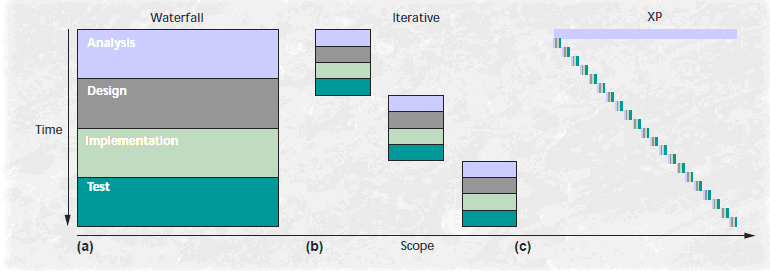
\includegraphics[width=\linewidth]{developmentMethodologies.png}
				\caption{Waterfall vs Iterative vs Extreme Programming methodologies.}
				\label{fig:developmentMethodologies}
			\end{figure}
		
		\subsection{Client Updates}
			\paragraph\indent
			Since Subtrop is located in Tzaneen it would be more practical to perhaps have Skype/Team Viewer meetings to do demos of the current progress of the system. Less frequent face-to-face meeting could be arranged in order for Subtrop and developers (students) to discuss important milestones in the project, should it be necessary.
			
		\subsection{Initial Ideas}
			\paragraph\indent
		
		\subsection{Potential Technologies}
			\paragraph\indent
		
		\subsection{Deliverables}
			\paragraph\indent
			A-Cube-N will provide all the source code in order to join Subtrop in making this software available for other subtropical farmers by means of open source. We will also provide detailed documentation on the system to facilitate future developments. And finally we will provide a user manual that will provide instructions on how the system is used and how it is set up.
\end{document}
